\documentclass[a4paper, 12pt]{article} % тип документа

%%%Библиотеки
	%\usepackage[warn]{mathtext}	
	\usepackage[T2A]{fontenc}   %Кодировка
	\usepackage[utf8]{inputenc} %Кодировка исходного текста
	\usepackage[english, russian]{babel} %Локализация и переносы
	\usepackage{caption}
	\usepackage{listings}
	\usepackage{amsmath, amsfonts, amssymb, amsthm, mathtools}
	\usepackage[warn]{mathtext}
	\usepackage[mathscr]{eucal}
	\usepackage{wasysym}
	\usepackage{graphicx} %Вставка картинок правильная
	\DeclareGraphicsExtensions{.pdf,.png,.jpg}
	\graphicspath{ {images/} }
	
	\setlength{\parskip}{0.5cm}
	
	\usepackage{pgfplots}
	\usepackage{indentfirst}
	\usepackage{float}    %Плавающие картинки
	\usepackage{wrapfig}  %Обтекание фигур (таблиц, картинок и прочего)
	\usepackage{fancyhdr} %Загрузим пакет
	\usepackage{lscape}
	\usepackage{xcolor}
	\usepackage[normalem]{ulem}
	\usepackage{wasysym}
	
	\usepackage{titlesec}
	\titlelabel{\thetitle.\quad}

	\usepackage{hyperref}
	\newenvironment{comment}{}{}

%%%Конец библиотек

%%%Настройка ссылок
	\hypersetup
	{
		colorlinks = true,
		linkcolor  = blue,
		filecolor  = magenta,
		urlcolor   = blue
	}
%%%Конец настройки ссылок


%%%Настройка колонтитулы
	\pagestyle{fancy}
	\fancyhead{}
	\fancyhead[L]{2.4.1}
	\fancyhead[R]{Старченко Иван, группа Б01-005}
	\fancyfoot[C]{\thepage}
%%%конец настройки колонтитулы

\begin{document}

%\maketitle
%\thispagestyle{empty}

%\newpage
\setcounter{page}{1}

\begin{center}
  \LARGE{Лабораторная работа 2.1.4}\\[0.2cm]
  \LARGE{Определение теплоемкости твердых тел}\\[0.2cm]
  \large{10 Марта 2021 г.}\\[0.2cm]
  \large{Старченко Иван Александрович}\\[0.2cm]
\end{center}


						%%%%Начало документа%%%%


\textbf{Цель работы:} 1) измерение количества подведенного тепла и вызванного им нагрева твердого тела; 2) определение теплоемкости по экстраполяции отношения $\dfrac {\Delta Q}{\Delta T}$ к нулевым потерям тепла.

\textbf{В работе используются:} калориметр с нагревателем и термометром cопротивления; амперметр; вольтметр;B мост постоянного тока; источ- ник питания 36 В.


\section{Теоретическое введение}

В предлагаемой работе измерение теплоёмкости твёрдых тел производится по обычной схеме. Исследуемое тело помещается в калориметр. Измеряется $\Delta Q$ --— количество тепла, подведённого к телу, и $\Delta T$ --— изменение температуры тела, произошедшее в результате подвода тепла. Теплоёмкость определяется по формуле
\begin{equation}	
	C = \dfrac{\Delta Q}{\Delta T}
\end{equation}

Температура исследуемого тела надежно измеряется термометром сопротивления, а определение количества тепла, поглощенного телом, обычно вызывает затруднение. В реальных условиях не вся энергия $P \Delta t$, выделенная нагревателем, идет на нагревание исследуемого тела и калориметра, часть ее уходит из калориметра благодаря теплопроводности его стенок. Оставшееся в калориметре количество тепла $\Delta Q$ равно
\begin{equation}
	\Delta Q = P\Delta t - \lambda \left( T - T_{\text{к}} \right) \Delta t,
\end{equation}

где $P$ -- мощность нагревателя, $\lambda$ -- коэффициент теплоотдачи стенок, $T$ -- температура тела, $T_{\text{к}}$ -- комнатная температура, $ \Delta t$ -- время, в течение которого идет нагревание.

Из уравнений (1) и (2) получаем
\begin{equation}
	C = \dfrac{P - \lambda(T - T_{\text{к}})}{\Delta T / \Delta t}
\end{equation}

Формула (3) является основной расчетной формулой работы. Она определяет теплоемкость тела вместе с калориметром. Теплоемкость калориметра измеряется отдельно и вычитается из результата.

С увеличением температуры исследуемого тела растет утечка энергии, связанная с теплопроводностью стенок калориметра. Из формулы (2) видно, что при постоянной мощности нагревателя по мере роста температуры количество тепла, передаваемое телу, уменьшается и, следовательно, понижается скорость изменения его температуры.

Погрешности, связанные с утечкой тепла, оказываются небольшими, если не давать телу заметных перегревов и проводить все измерения при температурах, мало отличающихся от комнатной. Однако при небольших перегревах возникает большая ошибка при измерении $\Delta T = T - T_\text{к}$, и точность определения теплоемкости не возрастает. Чтобы избежать этой трудности, в работе используется следующая методика измерений. Зависимость скорости нагревания тела $\Delta T / \Delta t$ от температуры измеряется в широком интервале изменения температур. По полученным данным строится график:
\begin{equation}
	\dfrac{\Delta T}{\Delta t} = f(T)
\end{equation}

Этот график экстраполируется к температуре $T = T_{\text{к}}$, и таким образом определяется скорость нагревания при комнатной температуре $(\Delta T / \Delta t)_{T_{\text{к}}}$. Подставляя полученное выражение в формулу (3) и замечая, что при $T = T_{\text{к}}$ член $\lambda(T - T_{\text{к}})$ обращается в ноль, получаем
\begin{equation}
	C = \dfrac{P}{(\Delta T / \Delta t)_{T_{\text{к}}}}
\end{equation}

Температура измеряется термометром сопротивления, представляющим собой медную проволоку, намотанную на теплопроводящий каркас внутренней стенки калориметра (рис. 1). Сопротивление проводника изменяется с температурой по закону
\begin{equation}
    R_{T} = R_{0}(1 + \alpha \Delta T)
\end{equation}
    
где $R_{T}$ -- сопротивление термеметра про $T  ^{\circ}C$, $R_{0}$ -- его сопротивление при $0  ^{\circ}C$, $\alpha$ -- температурный коэффициент сопротивления. 

Дифференцируя (6) по времени, найдем
\begin{equation}
	\dfrac{dR}{dt} = R_{0}\alpha \dfrac{dT}{dt},
\end{equation}

Выразим сопротивление $R_{0}$ через исмеренное значение $R_{\text{к}}$ -- сопротивление термометра при комнатной температуре. Согласно (6), имеем
\begin{equation}
	R_{0} = \dfrac{R_{\text{к}}}{1 + \alpha \Delta T_{\text{к}}}
\end{equation}

\begin{figure}[h]
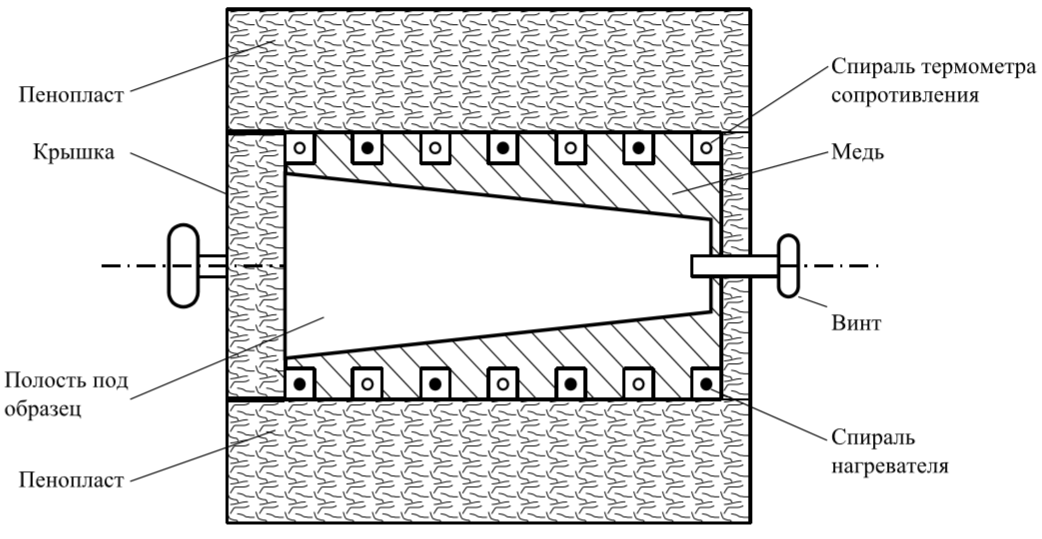
\includegraphics[scale = 0.62]{call.png}
\caption{"Схема устройства калориметра"}
\label{fig:image}
\end{figure}

\newpage
Подставляя (7) и (8) в (5), найдем
\begin{equation}
	C = \dfrac{P\cdot R\cdot \alpha}{\left(\dfrac{dR}{dt}\right)_{T_{\text{к}}}(1 + \alpha \Delta T_{\text{к}})}
\end{equation}

 Входящий в формулу температурный коэффициент сопротивления меди равен $\alpha = 4,28 \cdot 10^{-3}~\text{К}^{-1}$, все остальные величины определяются экспериментально. 


\section{Эксперементальная установка}

\begin{wrapfigure}[8]{p}{0.30\linewidth} 
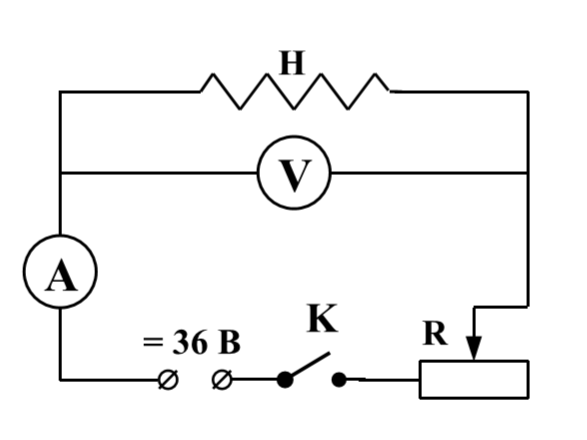
\includegraphics[scale = 0.28]{chema.png}
\caption{"Схема включения нагревателя"}
\label{fig:image}
\end{wrapfigure}

Установка состоит из калориметра с пенопластовой изоляцией, помещенного в ящик из многослойной клееной фанеры. Внутренние стенки калориметра выполненым из материала с высокой теплопроводностью. Надежность теплового контакта между телом и стенками обеспечивается их формой: они имеют вид усеченных конусов и плотно прилегают друг к другу. 


В стенку калориметра вмонтированы электронагреватель и термометр сопротивления. Схема включения нагревателя изображения на рис.2. Система реостатов позволяет установить нужную силу тока в цепи нагревателя. По амперметру и вольтметру определяется мощность, выделяемая в нагревателе. Величина сопротивления термометра измеряется мостом постоянного тока.

\section{Ход работы}

Настроим мост, а также измерим сопротивление термометра при комнатной температуре. Затем настроим нагреватель. Настройка оборудования закончена.

При неизменной мощности нагревателя опрелелите зависимость сопротивления термометра от времени для пустого калориметра $R_{\text{T}} = R(t)$. Заполним таблицу с полученными данными.

\FloatBarrier
\begin{center}
	\begin{table}[h]
	\begin{tabular}{| c | c | c | c | c | c | c | c | c | c |} 
	\hline
	$R,~$ Ом & 18,08 & 18,18 & 18,28 & 18,38 & 18,48 & 18,58 & 18,68 & 18,78 & 18,88  \\ \hline
	$t,~$ с & 0 & 92 & 187 & 289 & 398 & 513 & 638 & 766 & 904\\ \hline \hline
	$R,~$ Ом & 18,98 & 19,08 & 19,18 & 19,28 & 19,38 & 19,48 &&&  \\ \hline
	$t,~$ с & 1049 & 1202 & 1362 & 1538 & 1723 & 1914 &&& \\
	\hline
	\end{tabular}
	
	\caption{ Измерение зависимости сопротивления от времени для пустого калориметра.}
	\end{table}
\end{center}
\FloatBarrier

Аналогично получим таблицу зависмости сопротивления для латуни и алюминия.

\FloatBarrier
\begin{center}
	\begin{table}[h]
	\begin{tabular}{| c | c | c | c | c | c | c | c | c | c |} 
	\hline
	$R,~$ Ом & 18,08 & 18,18 & 18,28 & 18,38 & 18,48 & 18,58 & 18,68 & 18,78 & 18,88  \\ \hline
	$t,~$ с & 0 & 108 & 224 & 348 & 481 & 619 & 772 & 935 & 1112 \\ \hline \hline
	$R,~$ Ом & 18,98 & 19,08 & 19,18 & 19,28 & 19,38 & 19,48 &&&  \\ \hline
	$t,~$ с & 1294 & 1488 & 1701 & 1927 & 2157 & 2389  &&& \\
	\hline
	\end{tabular}
	
	\caption{ Измерение зависимости сопротивления от времени для алюминия.}
	\end{table}
\end{center}
\FloatBarrier
 
\FloatBarrier
\begin{center}
	\begin{table}[h]
	\begin{tabular}{| c | c | c | c | c | c | c | c | c | c |} 
	\hline
	$R,~$ Ом & 18,08 & 18,18 & 18,28 & 18,38 & 18,48 & 18,58 & 18,68 & 18,78 & 18,88  \\ \hline
	$t,~$ с & 0 & 135 & 274 & 421 & 576 & 741 & 913 & 1094 & 1285\\ \hline \hline
	$R,~$ О & 18,98 & 19,08 & 19,18 & 19,28 & 19,38 & 19,48 &&&  \\ \hline
	$t,~$ с & 1483 & 1693 & 1909 & 2135 & 2371 & 2619 &&& \\
	\hline
	\end{tabular}
	
	\caption{ Измерение зависимости сопротивления от времени для латуни.}
	\end{table}
\end{center}
\FloatBarrier

Изобразим полученные точки на графике и проведем через них плавную кривую. Затем разделим полученный график на 14 отрезков, найдя на каждом найдя коэффициент наклона по формуле (10). Полученные значени нанесем на график с помощью Matlab(график приведен в самом конце). Не забудем проэкстраполировать к точке $R_{\text{Т}} = R_{\text{К}}$
\begin{equation}
	\dfrac{dR}{dt}\approx\dfrac{R(t_{2}) - R(t_{1})}{t_{2} - t_{1}},
\end{equation}

Затем найдем теплоемкость пустого калориметра ($C_0$) по формуле (9). Аналогично найдем теплоемкости для латунного и алюминиевого тела, при этом учтя поправки на незамкнутость системы по следующей формуле.

\begin{equation}
	C_{1,2} = C^{'}_{1,2} - C_0,
\end{equation}
Где $C_{1,2} $ -- искомые теплоемкости без учета калориметра, $C^{'}_{1,2}$ -- полученные из графика теплоемкости с учетом калориметра, $C_0$ -- теплоемкость калориметра.

Далее посчитаем удельную и молярную теплоемкость по формулам:

\begin{equation}
	c_{1,2} = \frac{C_{1,2}}{m_{1,2}},~~~~~~~~~~ C_{\mu_1, \mu_2} = c_{1,2} \cdot \mu_{1, 2}
\end{equation}

\section{Обработка данных}

С помощью Matlab получим уравнения апроксимирующих прямых. В данном случае я воспоьзовался аппроксимацией полином второй степени, так как коэффициент при кубе в каждом из случаев $<< 1$.
Найдем $\bigg(\dfrac{dR}{dt}\bigg)$ при $R_k = 18.08 $ Ом в кадом из случаев:	

\begin{equation}
	\bigg(\frac{dR_{\text{кал}}}{dt}\bigg) = 0,0001R_{\text{к}}^2 - 0,0056R_{\text{к}} + 0,700 = 14,21 \cdot 10^{-4}~ \dfrac{\text{Ом}}{\text{с}}.,
\end{equation}
\begin{equation}
	\bigg(\frac{dR_{\text{лат}}}{dt}\bigg) = 0,0002R_{\text{к}}^2 - 0,0074R_{\text{к}} + 0,694 = 9,84 \cdot 10^{-4}~ \dfrac{\text{Ом}}{\text{с}} ,
\end{equation}
\begin{equation}
	\bigg(\frac{dR_{\text{алм}}}{dt}\bigg) = 0,0001R_{\text{к}}^2 - 0,0036R_{\text{к}} + 0,333 = 9,01 \cdot 10^{-4}~ \dfrac{\text{Ом}}{\text{с}}.
\end{equation}

Погрешности полученные в Matlab:
\begin{equation}
\sigma_{\frac{dR_{\text{кал}}}{dt}} = 0.91 \cdot 10^{-4}\ \frac{\text{Ом}}{\text{с}}, ~~~~~~~~~~~~~~
\varepsilon_{\frac{dR_{\text{кал}}}{dt}} = 6,4\ \%
\end{equation}
\begin{equation}
\sigma_{\frac{dR_{\text{кал}}}{dt}} = 0.72 \cdot 10^{-4}\ \frac{\text{Ом}}{\text{с}}, ~~~~~~~~~~~~~~
\varepsilon_{\frac{dR_{\text{кал}}}{dt}} = 7,32\ \%
\end{equation}
\begin{equation}
\sigma_{\frac{dR_{\text{кал}}}{dt}} = 0,51 \cdot 10^{-4}\ \frac{\text{Ом}}{\text{с}}, ~~~~~~~~~~~~~~
\varepsilon_{\frac{dR_{\text{кал}}}{dt}} = 5,66\ \%
\end{equation}

Теперь с помощью формулы (9) найдем теплоемкости.
\begin{equation}
	C_{\text{кал}} = 588,5\ \frac{\text{Дж}}{\text{К}}
\end{equation}
\begin{equation}
	C^{'}_{\text{алм}} = 849,3\ \frac{\text{Дж}}{\text{К}}
\end{equation}
\begin{equation}
	C^{'}_{\text{лат}} = 927,6\ \frac{\text{Дж}}{\text{К}}
\end{equation}

Погрешности полученные в Matlab:
\begin{equation}
\sigma_{C_{\text{кал}}} = 41.1\ \frac{\text{Дж}}{\text{К}}, ~~~~~~~~~~~~~~
\varepsilon_{C_{\text{кал}}} = 7,0\ \%
\end{equation}
\begin{equation}
\sigma_{C^{'}_{\text{алм}}} = 66,5\ \frac{\text{Дж}}{\text{К}}, ~~~~~~~~~~~~~~
\varepsilon_{C^{'}_{\text{алм}}} = 7,0\ \%
\end{equation}
\begin{equation}
\sigma_{C^{'}_{\text{лат}}} = 53,6\ \frac{\text{Дж}}{\text{К}}, ~~~~~~~~~~~~~~
\varepsilon_{C^{'}_{\text{лат}}} = 5,8\ \%
\end{equation}

Вычтем из полученных теплоемкостей теплоемкость пустого калориметра
\begin{equation}
	C_{\text{алм}} = 260,8\ \frac{\text{Дж}}{\text{К}}
\end{equation}
\begin{equation}
	C_{\text{лат}} = 339,1\ \frac{\text{Дж}}{\text{К}}
\end{equation}

Погрешности полученные в Matlab:
\begin{equation}
\sigma_{C_{\text{aлм}}} = 25.1\ \frac{\text{Дж}}{\text{К}}, ~~~~~~~~~~~~~~
\varepsilon_{C_{\text{алм}}} = 9,6\ \%
\end{equation}
\begin{equation}
\sigma_{C_{\text{лат}}} = 12.5\ \frac{\text{Дж}}{\text{К}}, ~~~~~~~~~~~~~~
\varepsilon_{C_{\text{лат}}} = 3.7\ \%
\end{equation}



Найдем удельнуютеплоемкость по формуле (12):
\begin{equation}
	c_{\text{алм}} = \frac{260,8}{294,2\cdot 10^{-3}} = 886,5\ \frac{\text{Дж}}{\text{К}\cdot \text{кг}}
\end{equation}
\begin{equation}
	c_{\text{лат}} = \frac{339,1}{875,5\cdot 10^{-3}} = 387,3\ \frac{\text{Дж}}{\text{K}\cdot \text{кг}}
\end{equation}

Погрешности полученные в Matlab:
\begin{equation}
\sigma_{c_{\text{алм}}} = 43.3\ \frac{\text{Дж}}{\text{К}}, ~~~~~~~~~~~~~~
\varepsilon_{C_{\text{алм}}} = 4.9\ \%
\end{equation}
\begin{equation}
\sigma_{c_{\text{лат}}} = 34.4\ \frac{\text{Дж}}{\text{К}}, ~~~~~~~~~~~~~~
\varepsilon_{C_{\text{лат}}} = 8,9\ \%
\end{equation}


Найдем молярную теплоемкость по формуле (12):
\begin{equation}
	C_{\mu \text{алм}} = 886,5\cdot 27\cdot 10^{-3}  = 23,9 \ \frac{\text{Дж}}{\text{К}\cdot \text{моль}}
\end{equation}
\begin{equation}
	C_{\mu \text{лат}} = 387,3\cdot 64,3\cdot 10^{-3} = 24,9 \ \frac{\text{Дж}}{\text{K}\cdot \text{моль}}
\end{equation}


Погрешности полученные в Matlab:
\begin{equation}
\sigma_{c_{\text{алм}}} = 103.86\ \frac{\text{Дж}}{\text{К}}, ~~~~~~~~~~~~~~
\varepsilon_{C_{\text{алм}}} = 4.9\ \%
\end{equation}
\begin{equation}
\sigma_{c_{\text{лат}}} = 49.45\ \frac{\text{Дж}}{\text{К}}, ~~~~~~~~~~~~~~
\varepsilon_{C_{\text{лат}}} = 8,9\ \%
\end{equation}

\section{Заключение}
В результате проделанного эксперимента были получены $c_{\text{алм}} = 886,5 \pm 43,3~\dfrac{\text{Дж}}{\text{К} \cdot \text{кг}}$, $c_{\text{лат}} = 387,3 \pm 34,4~\dfrac{\text{Дж}}{\text{К} \cdot \text{кг}}$. Табличные значения соответственно равны $c_{\text{а, табл}} = 920,0~\dfrac{\text{Дж}}{\text{К} \cdot \text{кг}}$ и $c_{\text{л, табл}} = 380,0~\dfrac{\text{Дж}}{\text{К} \cdot \text{кг}}$. Полученные значения лежат в пределах погрешности, что говрит о применимости данного метода.

\section{Список используемой литературы}

$\bullet$ Гладун А. Д. Лабораторный практикум по общей физике. Термодинамика и молекулярная физика\\

$\bullet$ \href{https://mipt.ru/education/chair/physics/S_II/lab/}{Описание лабораторных работ на кафедре общей физики МФТИ}

\newpage

\section{Графики}

\begin{figure}[h]
	\center{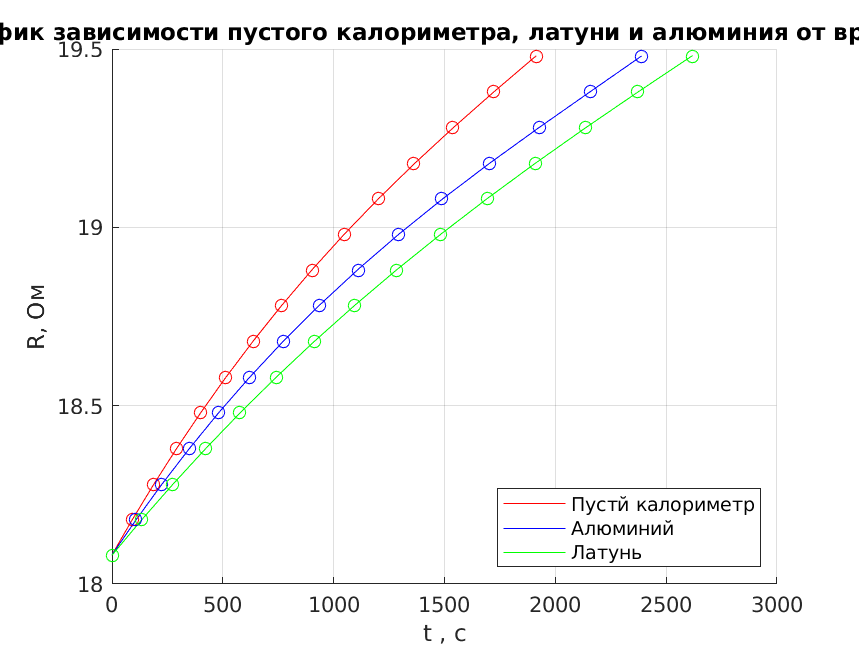
\includegraphics[scale = 0.68]{graph_1}}
\end{figure}

\begin{figure}[h]
	\center{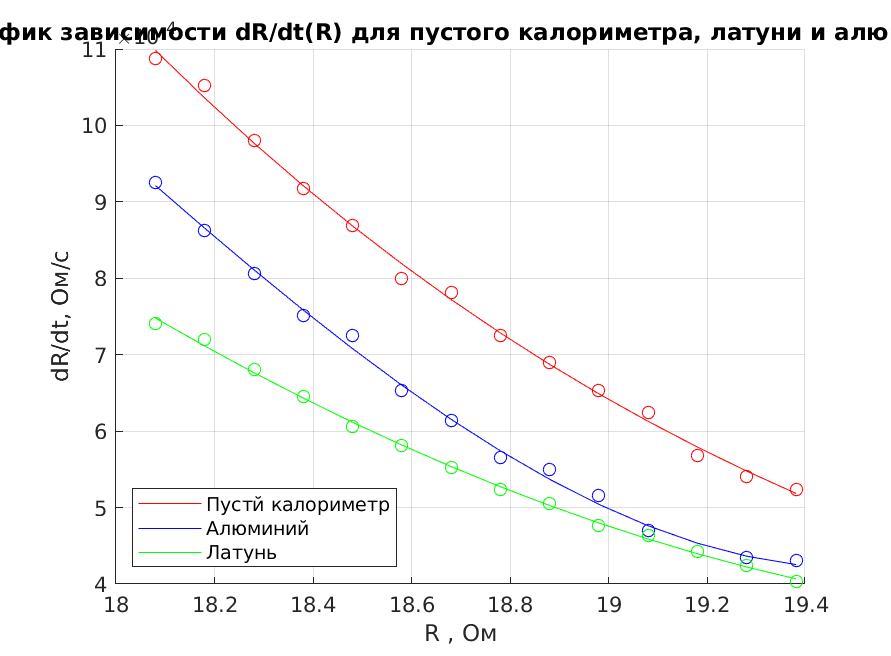
\includegraphics[scale = 0.68]{graph_2}}
\end{figure}




\end{document}
